\documentclass[handout]{beamer}

\usepackage{amsmath,amssymb,amsthm,array}
\usepackage{bm}
\usepackage{multirow}
\usepackage{multicol}
\usepackage{algorithm}
\usepackage{hyperref}
\usepackage{algorithmic}
\usepackage[normalem]{ulem}
\usepackage{fontspec}
\usepackage{numprint}
\usepackage{seqsplit}

\setmainfont{CMU Serif}
\setsansfont{CMU Sans Serif}
\newfontfamily{\greekfont}{CMU Serif}
\newfontfamily{\greekfontsf}{CMU Sans Serif}

\usetheme{metropolis}
 
\setbeamertemplate{navigation symbols}{}
\title{Ελλειπτικές καμπύλες}
\author{Παναγιώτης Γροντάς}
\date{11/12/2018}
\defbeamertemplate*{footline}{shadow theme}
{%
  \leavevmode%
  \hbox{
		\begin{beamercolorbox}[wd=.4\paperwidth,ht=2.5ex,dp=1.125ex,leftskip=.3cm,rightskip=.3cm plus1fil]{title in head/foot}%
			\usebeamerfont{title in head/foot} Elliptic Curves - Pairings  %
		\end{beamercolorbox}
		\begin{beamercolorbox}[wd=.5\paperwidth,ht=2.5ex,dp=1.125ex,leftskip=.3cm,rightskip=.3cm plus1fil]{title in head/foot}%
			\usebeamerfont{title in head/foot} \hfill \insertsection  %
		\end{beamercolorbox}
		\begin{beamercolorbox}[wd=.1\paperwidth,ht=2.5ex,dp=1.125ex,leftskip=.3cm plus1fil,rightskip=.3cm]{author in head/foot}%
			\usebeamerfont{author in head/foot}\insertframenumber\,/\,\inserttotalframenumber
		\end{beamercolorbox}%
  }%
  \vskip0pt%
}
\institute{ΕΜΠ - Κρυπτογραφία (2018-2019)}

 \hypersetup{
  pdfauthor={Panagiotis Grontas},
  pdftitle={EC-Pairings},
  colorlinks=true,
  urlcolor=blue,
  pdfborderstyle={/S/U/W 1}	% border style will be underline of width 1pt
}

\npthousandsep{ }
\setlength{\columnseprule}{0.4pt}
\begin{document}
\newcommand{\xor}{ \oplus }
\newcommand{\msg}{ \mathtt{M} }
\newcommand{\KEY}{ \mathtt{K} }
\newcommand{\CPH}{ \mathtt{C} }
\newcommand{\keygen}{\mathtt{KeyGen}}
\newcommand{\enc}{\mathtt{Enc}}
\newcommand{\dec}{\mathtt{Dec}}
\newcommand{\sign}{\mathtt{Sign}}
\newcommand{\ver}{$\mathcal{V} \ $}
\newcommand{\prv}{$\mathcal{P} \ $}
\newcommand{\verify}{\mathtt{Verify}}
\newcommand{\adv}{$\mathcal{A}$ }
\newcommand{\Hash}{\mathcal{H} }
\newcommand{\advb}{$\mathcal{B}$ }
\newcommand{\chal}{$\mathcal{C}$ }
\newcommand{\cs}{$\mathcal{CS}$}
\newcommand{\Zed}{\mathbb{Z}} 
\newcommand{\zns}{\mathbb{Z}^*_n}
\newcommand{\zs}[1]{\mathbb{Z}^*_{#1}}

\newcommand{\green}[1]{\textcolor{teal}{#1}}
\newcommand{\Green}[1]{\textcolor{Teal}{#1}}
\newcommand{\ForestGreen}[1]{\textcolor{ForestGreen}{#1}}
\newcommand{\blue}[1]{\textcolor{blue}{#1}}
\newcommand{\magenta}[1]{\textcolor{magenta}{#1}}
\newcommand{\cyan}[1]{\textcolor{cyan}{#1}}

\newcommand{\twopartdef}[4]
{ 
		\begin{cases}
			#1 , #2 \\
			#3 , #4
		\end{cases} 
}

\begin{frame}
	\titlepage
\end{frame}
	
\begin{frame}{Περιεχόμενα}
\begin{itemize}
\item Η ομάδα ελλειπτικών καμπυλών
\item Κρυπτογραφικά πρωτόκολλα
\item Pairings
\item Εφαρμογές PBC
\end{itemize}
\end{frame}

\section{Μαθηματικό υπόβαθρο}

\begin{frame}{Ελλειπτικές καμπύλες}
\begin{block}{Γενικά}
\begin{itemize}
\item Πλούσιο σε ιστορία μαθηματικό αντικείμενο
\begin{itemize}
	\item Πρώτη εμφάνιση Διόφαντος 3 αιώνας πΧ (ρητές ρίζες της $y^2 = x^3-x+9$)
	\item Μελέτη εδώ και 300 έτη \pause
\end{itemize}
\item Κρυπτογραφία: 80s (Neil Koblitz, Victor Miller) \pause
\item Βασίζεται στο πρόβλημα του Διακριτού Λογάριθμου \pause
\begin{itemize}
\item Αντικατάσταση του $\mathbb{Z}_{p}$ με σημεία τους \pause
\item Μόνο γενικευμένοι αλγόριθμοι DLP $O(2^\frac{\lambda}{2})$ - όχι υποεκθετικοί \pause
\item Ίδια επίπεδα ασφάλειας με μικρότερη παράμετρο - καλύτερη απόδοση\\
\begin{tabular}{cc}
RSA & EC \\
1024 & 160 \\
2048 & 224 \\
3072 & 256 \\
\end{tabular}
\end{itemize}
\end{itemize}
\end{block}
\end{frame}

\begin{frame}{Γενική μορφή}
Έστω $\mathbb F$ ένα σώμα.
\pause
\begin{block}{Ορισμός $\mathcal{E}(\mathbb{F})$}
Mια ελλειπτική καμπύλη $\mathcal{E}$ πάνω από το $\mathbb F$ είναι το σύνολο των σημείων  $(x,y) \in \mathbb F$, που ικανοποιούν την εξίσωση Weierstrass 
\begin{align*}
y^2+a_1xy+a_3y=x^3+a_2x^2+a_4x+a_6 \\  a_1, a_2, a_3, a_4, a_5, a_6 \in \mathbb{F}
\end{align*}  
 και  ένα στοιχείο $\mathcal O$, (- \emph{σημείο στο άπειρο})
\end{block}
\pause
\begin{block}{Πρακτικά} 
$
y^2=x^3+ax+b ,\ \ a, b \in \mathbb F\  
$

\end{block}
\end{frame}

\begin{frame}{Ελλειπτικές καμπύλες στο $\mathbb R$ (μορφή)}
\begin{figure}
\begin{tiny}
\begin{tabular}{cccc}
		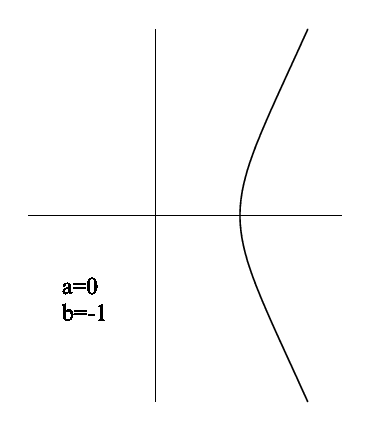
\includegraphics[scale=0.25]{qaz1.png} & $y^2 = x^3 - 1 $   & \pause 
		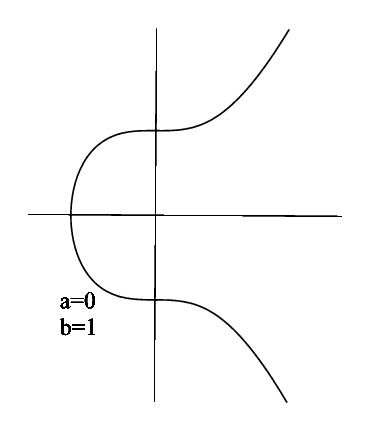
\includegraphics[scale=0.25]{qaz2.png} &  $y^2 = x^3 + 1 $ \pause \\       
		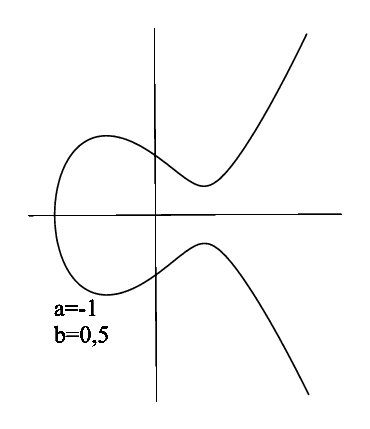
\includegraphics[scale=0.25]{qaz3.png} & $y^2 = x^3 - x +\frac{1}{2} $ & \pause 
		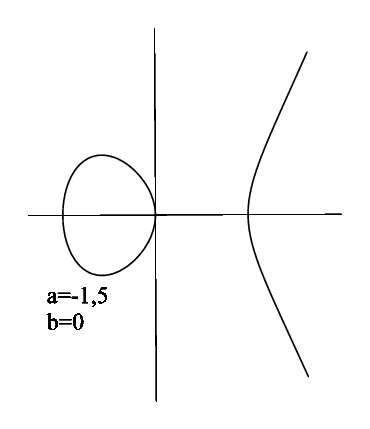
\includegraphics[scale=0.25]{qaz4.png}  &  $y^2 = x^3 - \frac{3}{2}x $
\end{tabular}
\end{tiny}
\end{figure}
\end{frame}

\begin{frame}{Παρατηρήσεις στη μορφή ελλειπτικών καμπυλών}

\begin{itemize}
\item Συμμετρία ως προς άξονα $x$ \pause
\item Συμπίεση σημείου: Αποθηκεύουμε τετμημένη και 1 bit για πάνω ή κάτω από τον άξονα των $x$ (δηλ.  $(x,0)$ ή $(x,1)$) \pause
  
\item \alert{Προς αποφυγή} Singular καμπύλες: Πολλαπλές ρίζες, σημεία τομής \\

\begin{figure}

\includegraphics[scale=0.3]{singular.png}
\end{figure}
Πρέπει $4a^3+27b^2 \neq 0$
\end{itemize}
\end{frame}

\begin{frame}{Ομάδα Σημείων Ελλειπτικής καμπύλης}
	Τα σημεία μιας ελλειπτικής καμπύλης αποτελούν αβελιανή ομάδα ως προς την πρόσθεση \pause
	\begin{itemize}
	\item ουδέτερο στοιχείο $\mathcal{O}$ \pause
	\item αντίθετο σημείου $P$ στην $\mathcal E(\mathbb{R})$:
	\begin{itemize}
		\item Αν $P=\mathcal O$, τότε  $-P=\mathcal O$
		\item Αν $P=(x,y)$ τότε $-P=(x,-y)$ \\(ανήκει στην $\mathcal E$ λόγω συμμετρίας)
	\end{itemize} \pause
	\item πρόσθεση: Για τρία σημεία $P,Q,R$ στην ίδια ευθεία: $P+Q+R=\mathcal O$
	\item πρόσθεση: προσεταιριστική και αντιμεταθετική
	\end{itemize}
\end{frame} 

\begin{frame}[allowframebreaks]{Πρόσθεση Σημείων}
(Γεωμετρική) Ερμηνεία

\magenta{Tο άθροισμα $P+Q$}
\begin{columns}
\column{0.5\textwidth}
Αν $P=\mathcal O$, τότε $\mathcal O+Q=Q$  

Αν $Q=-P$, τότε  $P+Q=\mathcal O$.  

Το σημείο $\mathcal O$. υπάρχει σε \textbf{κάθε κατακόρυφη}
\column{0.5\textwidth}
\begin{center}
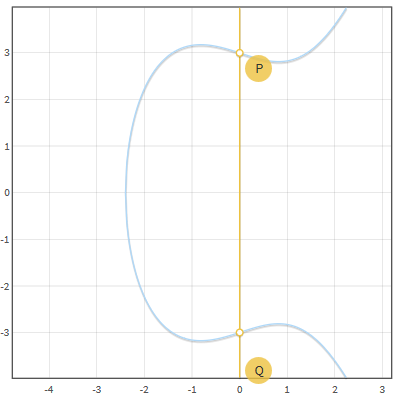
\includegraphics[scale=0.5]{add_opp.png} 
\end{center}

\end{columns}


\framebreak
\begin{columns}
\column{0.5\textwidth}
Αν $P = Q$ τότε:
\begin{itemize}
\item Θεωρούμε την εφαπτομένη στο $P$
\item Βρίσκουμε το σημείο τομής $R$ με την $\mathcal{E}$.
\item Βρίσκουμε το αντίθετο
\end{itemize}
\column{0.5\textwidth}
\begin{center}
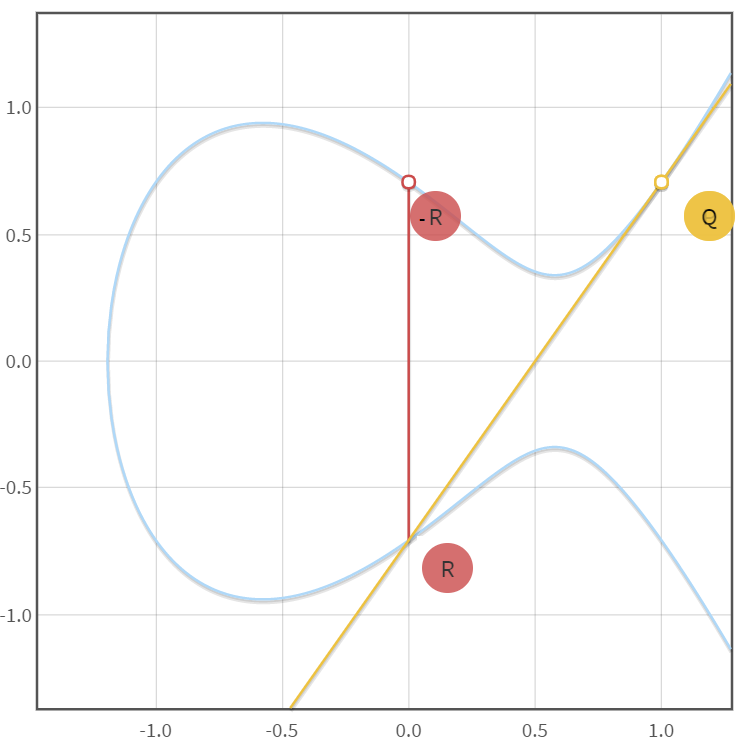
\includegraphics[scale=0.3]{add_same.png} 
\end{center}
\href{https://cdn.rawgit.com/andreacorbellini/ecc/920b29a/interactive/reals-add.html}{Elliptic Curve point addition}
\end{columns} 

\framebreak

\begin{columns}
\column{0.5\textwidth}
Αν $P \neq Q$ τότε:
\begin{itemize}
\item Θεωρούμε την $\overline{PQ}$
\item Αν υπάρχει σημείο τομής $R$ με την $\mathcal{E}$:
\begin{itemize}
	\item Βρίσκουμε το αντίθετο
\end{itemize}
\item Αν δεν υπάρχει σημείο τομής:
\begin{itemize}
	\item Σε ένα εκ των $P,Q$ η $\overline{PQ}$ θα εφάπτεται με την $\mathcal{E}$ 
	\item Βρίσκουμε το αντίθετο
\end{itemize} 
\end{itemize}
\column{0.5\textwidth}
\begin{center}
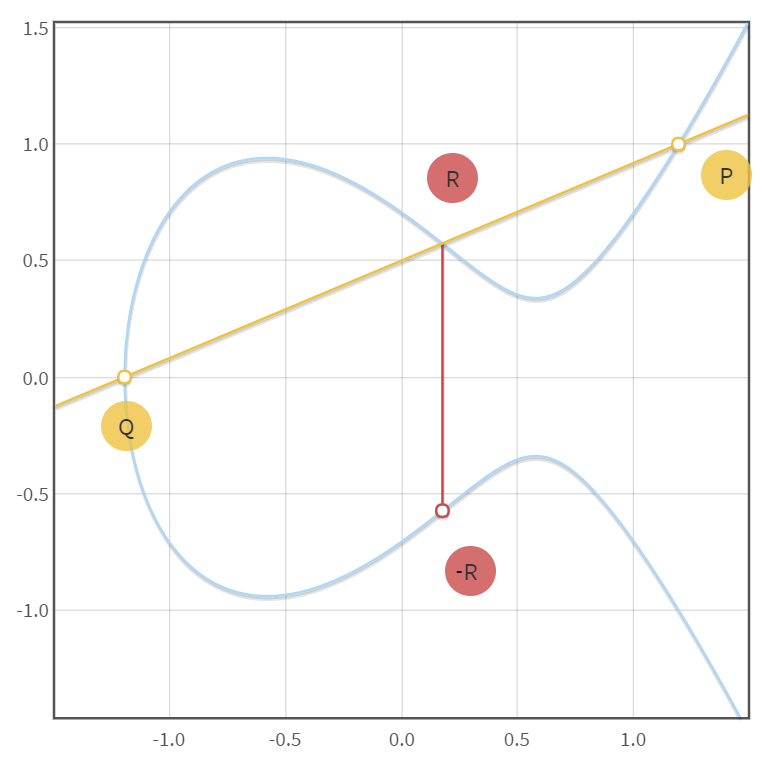
\includegraphics[scale=0.23]{add.png} \\
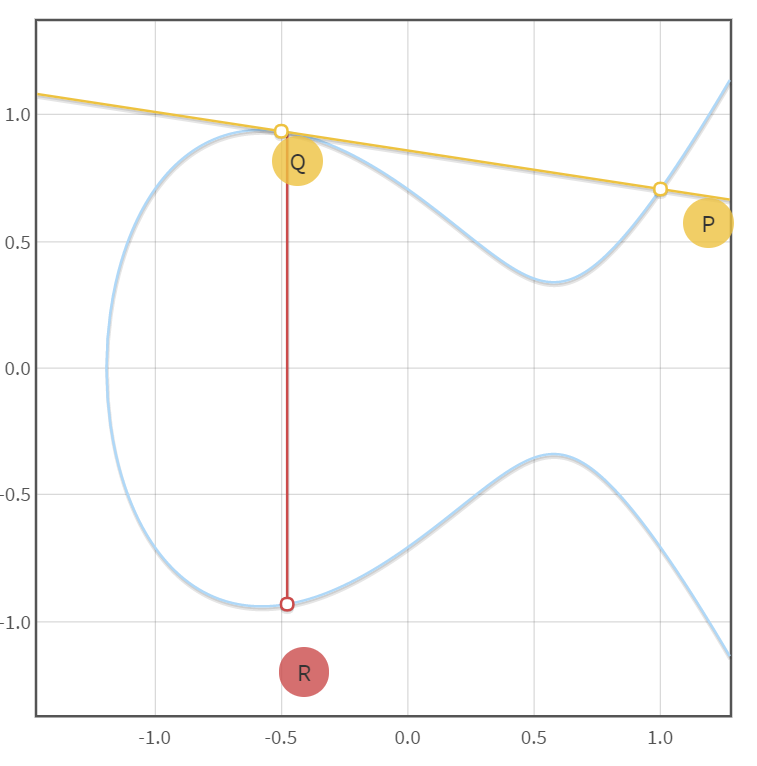
\includegraphics[scale=0.23]{add2.png} 
\end{center}
\end{columns}

\framebreak

\begin{block}{Αλγεβρική αναπαράσταση}
\begin{itemize}
	\item Συντελεστής ευθείας $\overline{PQ}$: $m = \frac{y_P-y_Q}{x_P-x_Q}$
	\item Εύρεση σημείου τομής $(x_R, y_R)$ με ελλειπτική καμπύλη
	\item Επίλυση τριτοβάθμιας εξίσωσης
\end{itemize}
\end{block}

\end{frame}


\begin{frame}{Πολλαπλασιασμός σημείου με ακέραιο $nP = P + P + \cdots + P$}

\begin{center}
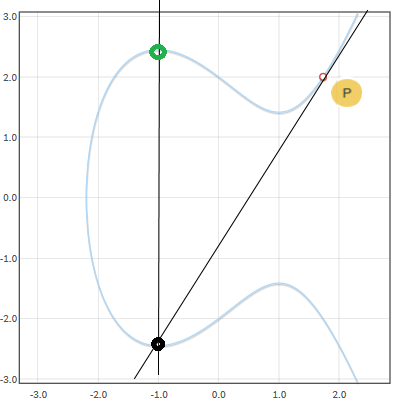
\includegraphics[scale=0.33]{p.png} 
\pause
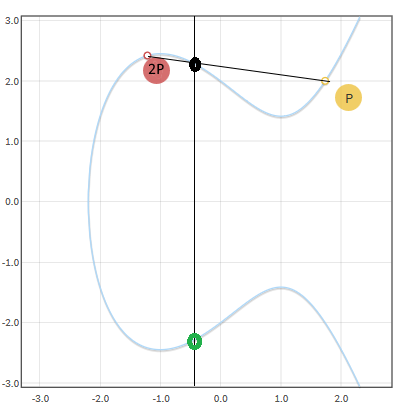
\includegraphics[scale=0.46]{2p.png} \\
\pause
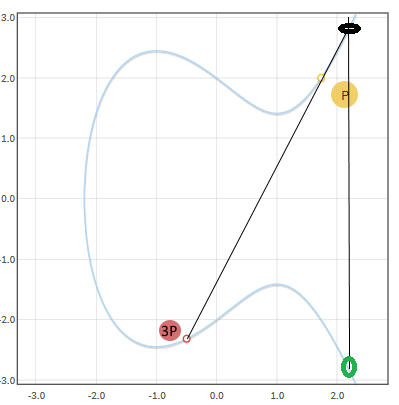
\includegraphics[scale=0.46]{3p.png} 
\pause
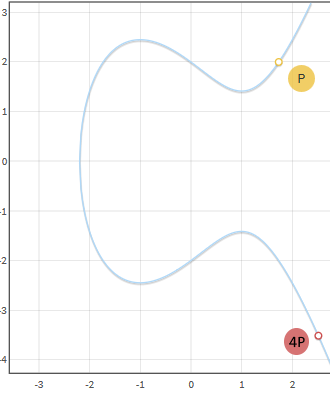
\includegraphics[scale=0.33]{4p.png} 
\end{center}
\end{frame}

\begin{frame}{Double and add}
\magenta{Υπολογισμός $nP$} \\
Απαιτούνται $n-1$ προσθέσεις \\ 

\green{Λύση:} Square and multiply - Double and add
\begin{align*}
17P = P + 16P \\
2P = P+P \\
4P= 2P+2P \\
8P= 4P+4P \\
16P= 8P+8P \\
\end{align*}
 
\end{frame}

\begin{frame}{Ελλειπτικές καμπύλες στο $\mathbb{F}_p$}

Ορισμός $\mathcal{E}(\mathbb{F}_p)$
\begin{align*}
 \mathcal E = \mathcal O \cup \{  y^2 = x^3 + ax +b \pmod{p},  \\
 (x,y) \in \mathbb{F}_p^2, (a,b) \in \mathbb{F}_p^2:  4a^3+27b^2 \neq 0 \pmod{p} \} 
\end{align*}
\pause
\medskip
Παράδειγμα: $y^2 = x^3-x+\frac{1}{2} \pmod{131}$\\
 \href{http://www.graui.de/elliptic-plot.htm}{Discrete Elliptic Curve Plotter}\\
\begin{center}
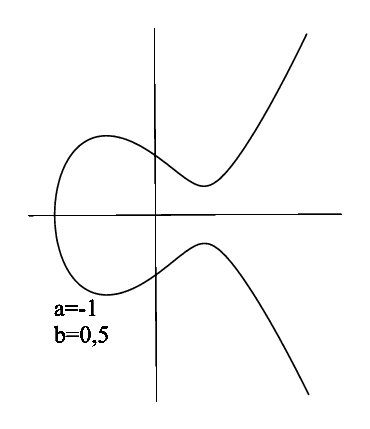
\includegraphics[scale=0.25]{qaz3.png} &
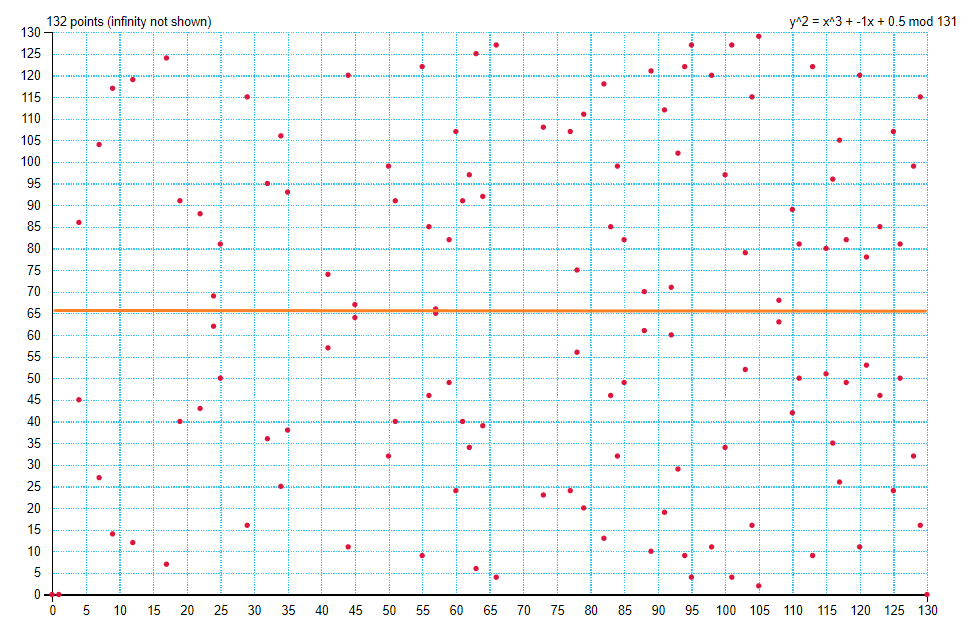
\includegraphics[scale=0.25]{ec997}
\end{center}

\end{frame}

\begin{frame}{Πρόσθεση σημείων στο $\mathbb{F}_p$}
Η ευθεία που συνδέει τα $P,Q,R$ επαναλαμβάνεται
\begin{center}
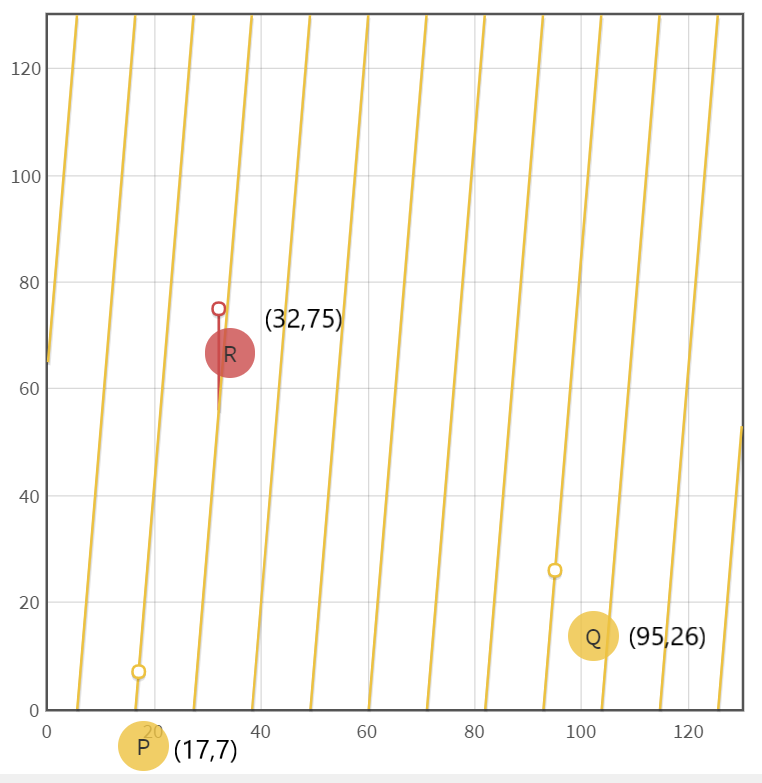
\includegraphics[scale=0.25]{addFp}
\end{center}
\end{frame}

\begin{frame}[allowframebreaks]{Η ομάδα των σημείων $\mathcal{E}(\mathbb{F}_p)$}

Εύρεση τάξης ομάδας

\begin{block}{Εκθετικός αλγόριθμος}
Δοκιμές όλων των $x \in \{0, \cdots, p-1\}$ για το ποια ικανοποιούν την εξίσωση της καμπύλης

Το πολύ $2p+1$ σημεία (συμμετρία + $\mathcal{Ο}$)
\end{block}

\begin{block}{Hasse bound}
$ p+1-2\sqrt{p} \leq\ | \mathcal E(\mathbb{F}_p) | \leq p+1+2\sqrt{p}$
\end{block}

\begin{block}{Υπολογισμός}
Αλγόριθμος Schoof σε $O(log(p))$ με βελτιώσεις Elkiens, Atkin (SEA)
\end{block}

\framebreak
\begin{block}{Κυκλικές υποομάδες}
Κάθε σημείο μιας καμπύλης $\mathcal{E}(\mathbb{F}_p)$ παράγει μια κυκλική υποομάδα
\end{block}
\pause
\begin{block}{Υπολογισμός τάξης υποομάδας σημείου στην $\mathcal{E}(\mathbb{F}_p)$}
Θεώρημα Lagrange:Η τάξη κάθε υποομάδας διαιρεί την τάξη της ομάδας
\pause

Υπολογισμός τάξης υποομάδας με σημείο βάσης (γεννήτορα) $P$
\begin{itemize}
\item Εύρεση τάξη ομάδας με αλγόριθμο Schoof \pause
\item Εύρεση των διαιρετών της τάξης, $d$ \pause
\item Εύρεση $min \{d: dP = \mathcal{O}\}$
\end{itemize}
\end{block}

\framebreak

\begin{block}{Εύρεση σημείων βάσης}
Θέλουμε γεννήτορες μεγάλων υποομάδων

\begin{itemize}
\item Επιλογή τάξης υποομάδας (μεγάλος πρώτος $q$): $q \mid |\mathcal{E}|$
\item Υπολογισμός cofactor $h=\frac{|\mathcal{E}|}{q}$
\item Επιλογή τυχαίου σημείου $P$
\item Υπολογισμός $G = hP$
\item Αν $G = \mathcal{O}$ επανάληψη
\end{itemize}
\end{block}

\end{frame}

\begin{frame}{Άλλα είδη καμπυλών}
	Βελτιστοποίηση πρόσθεσης σημείων και πολλαπλασιασμού σημείου με ακέραιο
	\begin{itemize}
		\item Koblitz curves: $y^2 +xy = x^3 +ax^2+1, a \in \{ 0,1 \}$
		\item Binary curves: $y^2 +xy = x^3 +x^2+b, b \in \mathbb{Z}$
		\item Edwards curves:  $y^2 +x^2 = 1+dx^2y^2, d \in \{ 0,1 \}$ (προστασία από side channels)
	\end{itemize}
\end{frame}

\begin{frame}{Πρόβλημα ECDLP}
\green{\emph{Δίνονται}}: 

\begin{itemize}
\item Μία ελλειπτική καμπύλη $\mathcal E$ ορισμένη πάνω από το $\mathbb{F}_p$ ($p,a,b,\# \mathcal E$)
\item Μία μεγάλη υποομάδα της με τάξη $q$ 
\item ένα σημείο βάσης $G$  και  
\item ένα σημείο  $Y$. 
\end{itemize}
\alert{\emph{Ζητείται}}:
Να βρεθεί, αν υπάρχει, ακέραιος $x$ τέτοιος ώστε $xG=Y$.

\pause
\begin{block}{Εικασία}
Το πρόβλημα ECDLP είναι υπολογιστικά απρόσιτο
\end{block}
\pause
\alert{Όχι σε κάθε καμπύλη}: 
\begin{itemize}
	\item MOV's attack (pairings) - υποεκθετικό DLP
	\item Smart's attack ($\#\mathcal{E}(\mathbb{F}_p)=p$) - πολυωνυμικό DLP
\end{itemize} 
\end{frame}


\begin{frame}{Επιλογή Καμπύλης}
	Συνέπεια: Δεν προτείνεται η παραγωγή καμπυλών, αλλά η χρήση έτοιμων\\
	\pause
	\alert{Πρόβλημα:} Μια καμπύλη $(p,a,b,\# \mathcal{E},q,G)$ - είναι ασφαλής (;)
	\pause
	\begin{block}{Επαληθευσιμότητα: Εγγύηση ότι δεν είναι 'πειραγμένη'}
	\begin{itemize}
	\item Επιλογή τυχαίου αριθμού $s$
	\item Υπολογισμός $h=\mathcal{H}(s)$
	\item Παραγωγή των $a,b,G$ από το $h$
	\item Επαληθεύσιμο, αλλιώς $a,b,G$ από αντιστροφή της σύνοψης
	\end{itemize}
	\end{block}
	\pause
	\alert{Αλλά:} Πρέπει το $s$ να είναι πραγματικά τυχαίο!
	\begin{block}{Nothing up my sleeve}
	Το $s$ προέρχεται από ψηφία του $\pi$, $e, \quad$ τριγωνομετρικών αριθμών
	\end{block}
\end{frame}

\begin{frame}[allowframebreaks]{Πρότυπες καμπύλες}
\begin{block}{Πρότυπο \href{http://csrc.nist.gov/publications/fips/fips186-3/fips_186-3.pdf}{NIST FIPS186-3}}

15 ελλειπτικές καμπύλες. Οι πιο γνωστές:

\begin{itemize}  
\item \textbf{NIST P-256} ή \textbf{secp256r1} 
$y^2 = x^3-3x+b \bmod ( 2^{256} - 2^{224} + 2^{192} + 2^{96} - 1)$\\
με $b=$\numprint{41058363725152142129326129780047268409114441015993725554835256314039467401291}\\
\item \textbf{NIST P-384 }
$y^2 = x^3-3x+b \bmod (2^{384}- 2^{128} - 2^{96} + 2^{32} - 1)$\\
με $b=$\numprint{27580193559959705877849011840389048093056905856361568521428707301988689241309860865136260764883745107765439761230575}\\
\end{itemize} 

\alert{Φόβοι για υπονόμευση}
\end{block}

\framebreak
Χρήση στην γεννήτρια τυχαιότητας Dual\_EC\_DRBG (NIST)
\begin{block}{Dual\_EC\_DRBG}
Δίνεται η καμπύλη NIST P-256, γεννήτορας $P$, σημείο $Q$, seed $s$ \\
Θέσε $r = x_{sP}$ \\
Θέσε $s' = x_{rP}$ \\
Θέσε $t = x_{rQ}$ \\
Επιστροφή $LSB_{-16}(t)$\\
Επανάληψη με $s=s'$
\end{block}
\begin{center}
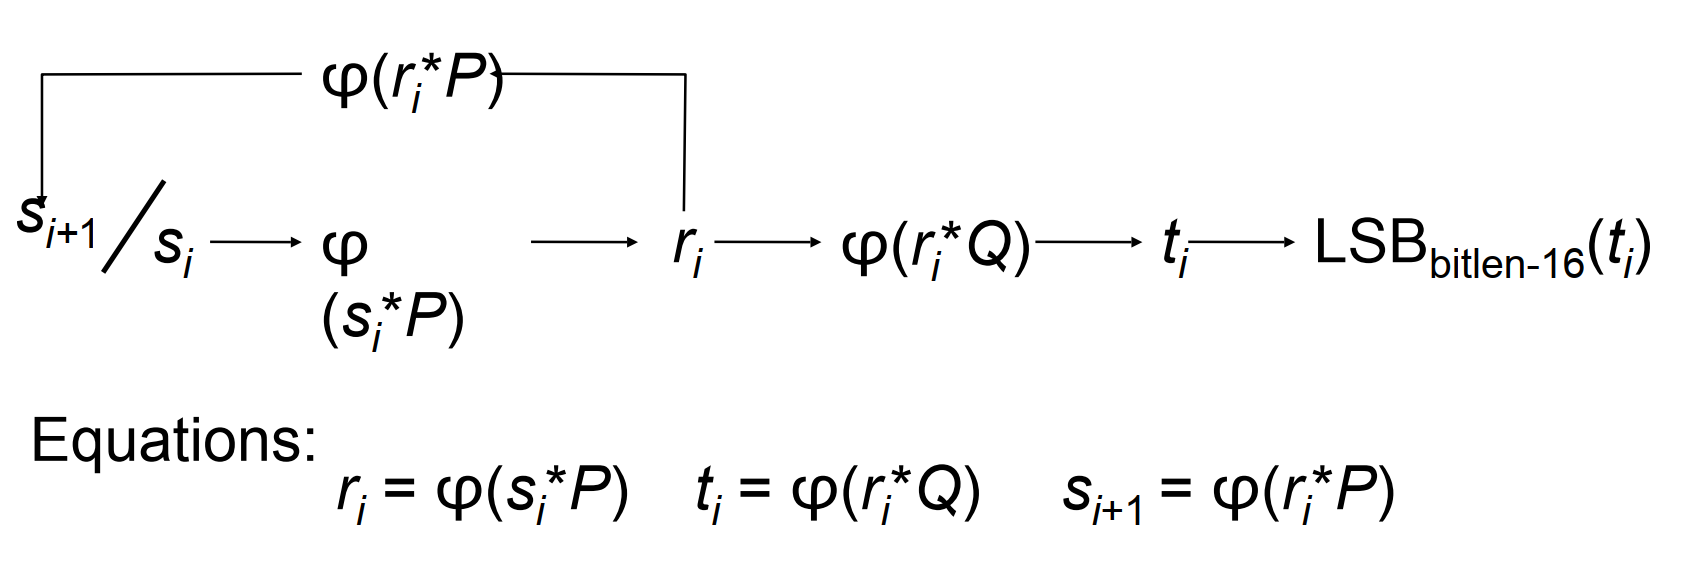
\includegraphics[scale=0.25]{Dual_EC_DRBG.png}
\end{center}
Προβλήματα (Shumow - Ferguson 2007)
\begin{itemize}
	\item Δεν αιτιολογείται η χρήση του $Q$
	\item Πολλά bits ως έξοδο τα οποία μπορούν να χρησιμοποιηθούν για την εύρεση του τελικού σημείου ($2^{16}$ έλεγχοι στην εξίσωση της καμπύλης)
	\item Πρόβλεψη των επόμενων εξόδων με βάση την σχέση $Q=eP$ (e backdoor)
\end{itemize}
 
\green{Εναλλακτικά}:\\
\textbf{secp256k1}  (OpenSSL, Bitcoin) \\
$y^2 = x^3+0x+7 \bmod (2^{256} - 2^{32} - 977)$ \\

\textbf{Curve25519} (OpenSSH) \\
$y^2 = x^3+486662 \cdot x^2+x \bmod (2^{255}-19) $
\end{frame}

\section{Κρυπτογραφικά πρωτόκολλα}
\begin{frame}[allowframebreaks]{Ανταλλαγή Κλειδιού ECDH}
\begin{block}{Στόχοι}
\begin{itemize}
\item Κατασκευή κοινού κλειδιού πάνω από δημόσιο κανάλι επικοινωνίας
\item Σε EC: Το κοινό κλειδί είναι σημείο της καμπύλης
\item Δημόσια επικοινωνία και συμφωνία σε σημείο $P$  μιας ελλειπτικής καμπύλης $\mathcal E$
\end{itemize}
\end{block}

Δημόσια Διαθέσιμες Παράμετροι: $(p,a,b,\# \mathcal E,q,G)$
\framebreak
\begin{block}{Πρωτόκολλο}
\begin{itemize}
\item H {Alice} επιλέγει έναν ακέραιο $a \in \{1, \cdots, q-1 \}$
\item Υπολογίζει το $aG \in \mathcal E$ και το δημοσιοποιεί.
\item Ο {Bob} επιλέγει έναν ακέραιο $b \in \{1, \cdots, q-1 \}$ και δημοσιοποιεί το $bG \in \mathcal E$
\item Το δημόσιο κλειδί που θα χρησιμοποιούν στη συνέχεια είναι το $P=a(bG)=b(aG) \in \mathcal E$
\end{itemize}
\end{block}

\end{frame}

\begin{frame}{Κρυπτογραφία Δημοσίου Κλειδιού}
\magenta{Παραλλαγή Κρυπτοσυστήματος ElGamal}

\textbf{Δημιουργία κλειδιών }
\begin{itemize}
\item Δημόσια Διαθέσιμες Παράμετροι: $(p,a,b,\# \mathcal E,q,G)$ \pause
\item Ιδιωτικό κλειδί: Ένας τυχαίος ακέραιος $x \in \{1, \cdots, q-1 \}$ \pause
\item Δημόσιο κλειδί: Το σημείο $Y=xG \in \mathcal{E}$ \pause
\end{itemize}

\textbf{Κρυπτογράφηση}
\begin{itemize}
\item Κωδικοποίηση μηνύματος ως σημείο $P_m$ της $\mathcal{E}$ \pause
\item Επιλέγεται ένας τυχαίος ακέραιος $k \in \{1, \cdots, q-1 \}$ \pause
\item Κρυπτογράφημα: $\enc(Y,m) = (kG,P_m+kY)$ \pause
\end{itemize}

\textbf{Αποκρυπτογράφηση}
\begin{itemize}
\item Υπολογισμός \[P_m+kY-x(kG)=P_m\] 
\end{itemize}

\end{frame}


\begin{frame}{Πρακτικά Θέματα}
Κωδικοποίηση μηνύματος σε σημείο
\begin{itemize}
\item 1ος τρόπος: Hashed Elgamal
\begin{itemize}
\item Χρήση συνάρτησης $\mathcal{H}: \mathcal{E} \rightarrow \mathcal{M}$
\item Κρυπτογράφηση: $\enc(Y,P_m) = (kG, m\oplus \mathcal{H}(kY))$
\end{itemize}
\item 2oς τρόπος
\begin{itemize}
\item Επιλογή τυχαίου $x_P$ και αντικατάσταση των bits χαμηλής τάξης του με το $m$
\item Επιλογή ενός από τα δύο πιθανά σημεία της καμπύλης
\item Αν δεν ανήκει τότε επανάληψη
\end{itemize}
\end{itemize}
\end{frame}


\begin{frame}[allowframebreaks]{Ψηφιακές Υπογραφές - ECDSA}

\textbf{Δημιουργία κλειδιών }
\begin{itemize}
\item Δημόσια Διαθέσιμες Παράμετροι: $(p,a,b,\# \mathcal{E},q,G)$
\item Ιδιωτικό κλειδί: Ένας τυχαίος ακέραιος $x \in \{1, \cdots, q-1 \}$
\item Δημόσιο κλειδί: Το σημείο $Y=xG \in \mathcal{E}$
\end{itemize}

\framebreak

\textbf{Υπογραφή}
\begin{itemize}
\item Υπολογισμός σύνοψης του μηνύματος $h = \mathcal{H}(M)$ και προσαρμογή της στο $[ 0, \cdots, q-1 ]$
\item Επιλογή τυχαίου αριθμού $k$ στο σύνολο $\{ 1, \cdots, q-1 \}$
\item Υπολογισμός του σημείου $P=kG=(x_P,y_P)$.
\item Υπολογισμός του $r = x_P \bmod q$
\item \alert{Αν $r = 0 \pmod{q}$ τότε επανάληψη με καινούριο $k$}.
\item Υπολογισμός του $s = k^{-1} (h + r \cdot x) \bmod{q}$
\item \alert{Αν $s=0$ τότε επανάληψη με καινούριο $k$}.
\item Η υπογραφή είναι το ζεύγος $(r,s)$
\end{itemize}

\framebreak
\textbf{Επαλήθευση}
\begin{itemize}
\item Υπολογισμός του $u_1 = s^{-1} h \bmod{q}$
\item Υπολογισμός του $u_2 = s^{-1} r \bmod{q}$
\item Υπολογισμός του σημείου $P' = u_1 G + u_2 Y$
\item H υπογραφή είναι έγκυρη αν $r = x_{P' } \pmod{q}$ 
\end{itemize}

\medskip
\textbf{Ορθότητα}: Υπολογισμός ίδιου σημείου με 2 τρόπους
\begin{itemize}
\item Υπογραφή $P=kG$
\item Επαλήθευση $P' = u_1 G + u_2 Y $
\end{itemize}
\begin{align*}
P' = u_1 G + u_2 Y = s^{-1} (h+rx) G = k(h+rx)^{-1}(h+rx)G = kG = P
\end{align*}

\framebreak
\alert{Ασφάλεια: Επιλογή διαφορετικού $k$ ανά υπογραφή}

Αλλιώς: Ανάκτηση ιδιωτικού κλειδιού!

\begin{block}{Επίθεση επανάληψης τυχαιότητας}
Δίνονται δύο υπογραφές $(r_1,s_1) (r_2,s_2)$

Παρατήρηση: $r_1 = r_2 = x__{kG}$

Τότε: $s_1 - s_2 = k^{-1}(h_1 - h_2) \pmod{q}$

Ανάκτηση $k = (h_1 - h_2)(s_1 - s_2)^{-1} \pmod{q}$

Ανάκτηση $x = (ks_1 - h_1){r^{-1}}$
\end{block}

\framebreak
Sony PlayStation 3 hack (2011): Υπογραφή όλων των παιχνιδιών με ίδιο $k$
\begin{center}
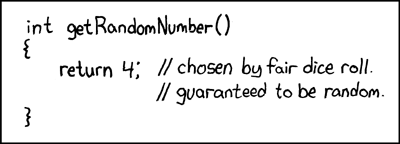
\includegraphics[scale=0.5]{random_number.png}

\href{https://xkcd.com/221/}{https://xkcd.com/221/}
\end{center}
\end{frame}


\begin{frame}[allowframebreaks]{Schnorr Signatures}

\textbf{Δημιουργία κλειδιών }
\begin{itemize}
\item Δημόσια Διαθέσιμες Παράμετροι: $(p,a,b,\# \mathcal{E},q,G)$
\item Ιδιωτικό κλειδί: Ένας τυχαίος ακέραιος $x \in \{1, \cdots, q-1 \}$
\item Δημόσιο κλειδί: Το σημείο $Y=xG \in \mathcal{E}$
\end{itemize}

\framebreak

\textbf{Υπογραφή Μηνύματος $m$}
\begin{itemize}
\item Επιλογή τυχαίου αριθμού $k$ στο σύνολο $\{ 1, \cdots, q-1 \}$
\item Υπολογισμός του σημείου $P=kG$.
\item Υπολογισμός του $s = k + x \cdot \mathcal{H}(P||Y||m)$
\item Η υπογραφή είναι το ζεύγος $(P,s)$ (σημείο και τιμή)
\end{itemize}

\framebreak

\textbf{Επαλήθευση υπογραφής στο $m$}
\begin{align*}
\verify(\mathcal{H},m,(P,s)) =\twopartdef{1}{ s \cdot G = P + \mathcal{H}(P||Y||m) \cdot Y}{0}{\text{αλλιώς}} 
\end{align*}

Ορθότητα:
\begin{align*}
s \cdot G &= (k + x \cdot \mathcal{H}(P||Y||m)) \cdot G \\
& = kG + xG \cdot \mathcal{H}(P||Y||m) \\
& = P + Y \cdot \mathcal{H}(P||Y||m)
\end{align*}

Βελτίωση απόδοσης: Batch validation (ακόμα και με διαφορετικά κλειδιά)
\begin{align*}
	\verify(\mathcal{H},(m_1, P_1,s_1), \cdots, (m_n,P_n,s_n)) : \\
	(s_1 + \cdots + s_n) \cdot G = \\
	P_1 + \mathcal{H}(P_1||Y_1||m_1) \cdot Y_1 + \cdots + P_n + \mathcal{H}(P_n||Y||m_n) \cdot Y_n
\end{align*}

\end{frame}


\section{Pairing Based Cryptography}

\begin{frame}{Ορισμός}
$\mathbb{G}_1, \mathbb{G}_2, \mathbb{G}_T$ πεπερασμένες κυκλικές ομάδες \pause

Ζεύξη (pairing-bilinear map): Μία \emph{αποδοτικά} υπολογίσιμη συνάρτηση 
$$e : \mathbb{G}_1 \times \mathbb{G}_2 \rightarrow \mathbb{G}_T$$
\pause
1) Διγραμμική (bilinear): 
$$e(g_1 \cdot g_2, h_1) = e(g_1,h_1) \cdot e(g_2,h_1) \text{και}$$
$$e(g_1,h_1 \cdot h_2) = e(g_1,h_1) \cdot e(g_1,h_2)$$
ή ισοδύναμα
$e(g^a,h^b) = e(g,h)^{ab} \quad \forall g \in \mathbb{G}_1, h \in \mathbb{G}_2 \ a,b \in \mathbb{Z}$
\pause

2) Μη εκφυλισμένη (non-degenerate): \\
Αν $\mathbb{G}=\langle g \rangle$ τότε $\mathbb{G}_T = \langle e(g,g) \rangle$

\end{frame}

\begin{frame}{Ορισμός (2)}
Μπορεί και $\mathbb{G}_1 = \mathbb{G}_2 = \mathbb{G}$

Συνήθως: 
$\mathbb{G}_1, \mathbb{G}_2, \mathbb{G} \subseteq \mathcal{E}(\mathbb{F}_p), \mathbb{G}_T \subseteq \mathbb{F}_{p^a}^*$ 
\pause

Συνέπεια ορισμού: Συμμετρία $e(g^a,g^b)  = e(g,g)^{ab} = e(g^b,g^a)$ \pause
\begin{block}{Pairings: ένα απλό παράδειγμα}
	$e(x,y) = 2^{xy}$ Τότε: \\
	$e(a,b+c) = 2^{a(b+c)}$ και:
	$e(a,b) \cdot e(a,c) = 2^{ab} \cdot 2^{ac} = 2^{a(b+c)}$
	Διαίσθηση: πολλαπλασιασμός σε κρυπτογραφημένες τιμές
\end{block}
\end{frame}

\begin{frame}{Ζεύξεις στην κρυπτογραφία}
	\begin{itemize}
		\item Στο $\mathbb{G}$ κάποια προβλήματα είναι δύσκολα, αλλά στο $\mathbb{G}_T$ μπορεί να είναι εύκολα \pause
		\item Λόγω της απεικόνισης $e$ μπορούμε να μεταβούμε αποδοτικά από την δύσκολη εκδοχή στην εύκολη \pause
		\item Χρήσιμη ασυμμετρία για την κατασκευή κρυπτογραφικών πρωτοκόλλων
		\item Πχ: Υπογραφές: \pause
		\begin{itemize}
			\item Κατασκευή	υπογραφής στο $\mathbb{G}$
			\item Επαλήθευση στο $\mathbb{G}_T$ μέσω του pairing
		\end{itemize} \pause
		\item Αρνητικές συνέπειες: Κάποια προβλήματα γίνονται ευκολότερα αν όχι εύκολα
	\end{itemize}
\end{frame}

\begin{frame}{Το DDHP είναι εύκολο...}
...\alert{αν υπάρχει pairing} \pause

Θέλουμε να ελέγξουμε αν $g^c = g^{ab}$, με δεδομένα τα $g^a,g^b, g^c$. \pause

Αποδοτικός υπολογισμός μέσω ζεύξης: $e(g^a, g^b) = e(g,g)^{ab}$ \pause

Σύγκριση με το $e(g,g^c)=e(g,g)^c$ 
\end{frame}

\begin{frame}{{Όχι όμως και το DLP...}}
...\alert{παρά την ύπαρξη pairing} \pause

Αντί για εύρεση $x$ από $g,g^x$ στην $\mathbb{G}$ (ελλειπτική καμπύλη)  \pause

εύρεση $x$ από $e(g,g),e(g,g^x)$ στην $\mathbb{G}_T$ (πεπερασμένο σώμα)  \pause

Το DLP έγινε ευκολότερο (υποεκθετικοί αλγόριθμοι), όχι όμως εύκολο (MOV - attack) \pause

Επιλογή μεγαλύτερης τιμής για παράμετρο ασφάλειας 
\end{frame}

\begin{frame}{Διγραμμικό Πρόβλημα Απόφασης Diffie-Hellman}
	Διαχωρίζονται στοιχεία του $\mathbb{G}_T$
	\begin{block}{BDDHP}
		\emph{Δίνονται}: δύο στοιχεία $h,g \in \mathbb{G}$ και τα στοιχεία $g^\alpha, g^\beta,  e(h,g)^c$.

		\pause
		\emph{Ζητείται}: Ισχύει $c = \alpha \beta$;
	\end{block} 
\end{frame}

\begin{frame}{Είδη pairings}
	\begin{itemize}
		\item Συμμετρικά 
		
		\item $e : \mathbb{G} \times \mathbb{G} \rightarrow \mathbb{G}_T$ (Weil pairing) \pause
		
		\item Ασύμμετρα 		
		$e : \mathbb{G}_1 \times \mathbb{G}_2 \rightarrow \mathbb{G}_T$ \pause
		\begin{itemize}
			\item Με εύκολο DDHP στο $\mathbb{G}_1$
			\item Χωρίς εύκολο DDHP στο $\mathbb{G}_1,\mathbb{G}_2$
			\item Tate pairing
		\end{itemize}
	\end{itemize}
	Διαφορετικές υποθέσεις ασφάλειας
\end{frame}

\section{Εφαρμογές PBC}
\begin{frame}{Τριμερής ανταλλαγή κλειδιού}
	Έστω κυκλική ομάδα με $\mathbb{G}=\langle g \rangle$ \pause
	
	Τρεις οντότητες $A,B,C$ με ζευγάρια ιδιωτικών - δημοσίων κλειδιών $(x_A, y_A=g^{x_A}),(x_B, y_B=g^{x_B}),(x_C, y_C=g^{x_C})$. \pause
	
	Μπορεί να συμφωνηθεί ένα κοινό κλειδί μεταξύ τους;
\end{frame}

\begin{frame}{Χωρίς pairings - σε 3 γύρους}
	\begin{enumerate}
		\item Ο $A$ στέλνει το $y_A$ στον $B$, ο $B$ στέλνει το $y_B$ στον $C$, ο $C$ στέλνει το $y_C$ στον $A$ (κυκλικά). \pause
		\item Ο $A$ υπολογίζει το $t_A = y_C^{x_A} = g^{x_Cx_A}$, o $B$ υπολογίζει το $t_B = y_A^{x_B} = g^{x_Bx_A}$ και ο $C$ υπολογίζει το $t_C = y_B^{x_C} = g^{x_Bx_C}$ \pause
		\item Ο $A$ στέλνει το $t_A$ στον $B$, ο $B$ στέλνει το $t_B$ στον $C$, ο $C$ στέλνει το $t_C$ στον $A$ (πάλι κυκλικά). \pause
		\item Όλοι υπολογίζουν το κοινό κλειδί ως εξής:
		\begin{itemize}
			\item Ο $A$ με $t_C ^ {x_A} = g^{x_Bx_Cx_A}$ \pause
			\item Ο $B$ με $t_A ^ {x_B} = g^{x_Cx_Ax_B}$ \pause
			\item Ο $C$ με $t_B ^ {x_C} = g^{x_Ax_Bx_C}$ \pause
		\end{itemize}
		\end{enumerate}
\end{frame}

\begin{frame}{Με pairings - σε 1 γύρο (Joux-2000)} 
Υποθέτουμε δύο ομάδες  $\mathbb{G}$, $\mathbb{G}_Τ$ με τάξη ένα πρώτο $q$ και μία συμμετρική διγραμμική ζεύξη $e : \mathbb{G} \times \mathbb{G} \rightarrow \mathbb{G}_T$.  \pause
\begin{itemize}
\item Όλοι οι συμμετέχοντες εκπέμπουν τα δημόσια κλειδιά τους $y_A=g^{x_A},y_B=g^{x_B},y_C=g^{x_C}$. \pause
\item Με την βοήθεια της ζεύξης το κοινό κλειδί μπορεί να υπολογιστεί ως εξής: 
\begin{itemize}
\item $e(g^{x_B},g^{x_C})^{x_A} = e(g,g)^{x_Bx_Cx_A}$ \pause
\item $e(g^{x_A},g^{x_C})^{x_B} = e(g,g)^{x_Ax_Cx_B}$ \pause
\item $e(g^{x_A},g^{x_B})^{x_C} = e(g,g)^{x_Ax_Bx_C}$
\end{itemize}
\end{itemize}
\end{frame}

\begin{frame}{Υπογραφές BLS}
	\begin{itemize}
		\item Boneh, Lynn και Shacham 2004
		\item Υπογραφές με βάση το DLP αλλά με μικρό μέγεθος
		\item Αντί για 2 στοιχεία, 1 στοιχείο με μέγεθος όσο η τάξη της ομάδας
	\end{itemize}
\end{frame}

\begin{frame}{Υπογραφές BLS - Ορισμός}
	\begin{itemize}
		\item \emph{Δημιουργία κλειδιών}: 
		$KeyGen(1^\lambda) = (\mathbb{G},\mathbb{G}_T, e, x, y)$ \pause
		\begin{itemize}
			\item Ομάδες $(\mathbb{G} = \langle g \rangle,\mathbb{G}_T)$ τάξης $q$ με δύσκολο CDH \pause
			\item $e: \mathbb{G} \times \mathbb{G} \rightarrow \mathbb{G}_T$ \pause
			\item Συνάρτηση σύνοψης: $\mathcal{H}:\{0,1\}^* \rightarrow \mathbb{G}$ \pause
			\item Κλειδί υπογραφής: $x \in_R \mathbb{Z}_q$ \pause
			\item Κλειδί επαλήθευσης: $y = g^x$
		\end{itemize}
		\item \emph{Υπογραφή}: 
		\begin{itemize}
			\item Υπολογισμός $h=\mathcal{H}(m)$ \pause
			\item Υπολογισμός $s = h^x$ \pause
			\item Επιστροφή $s \in \mathbb{G}$ 
		\end{itemize}
		\item \emph{Επαλήθευση}: 
		\begin{itemize}
			\item Υπολογισμός $h=\mathcal{H}(m)$ \pause
			\item Έλεγχος $e(g,s)==e(y,h)$
		\end{itemize}
	\end{itemize}	
\end{frame}

\begin{frame}{Υπογραφές BLS - Ιδιότητες} 
	\begin{block}{Ορθότητα:}
	$e(g,s) = e(g,h^x) = e(g,\mathcal{H}(m))^x$ και  \pause

	$e(y,h) = e(g^x,\mathcal{H}(m)) = e(g,\mathcal{H}(m))^x$  \pause
	\end{block}
	\begin{block}{Ασφάλεια:}
	Ανάγεται στο CDH στην $\mathbb{G}$
	\end{block} \pause
	\begin{block}{Aggregation:} 

	Χρήστες: $\{(x_i, y_i = g^{x_i}) \}_{i=1}^n$ , υπογραφές: $\{ s_i \}_{i=1}^n$ \pause

	Δημιουργία κοινής υπογραφής: $S = \prod_{i=1}^n s_i$ \pause

	Επαλήθευση: $\prod_{i=1}^n e(y_i,\mathcal{H}(m_i)) == e(g,S)$
	\end{block}	
\end{frame}

\begin{frame}{Identity based cryptography}
	\begin{itemize}
		\item Signatures:Shamir 1984 \pause
		\item Encryption:Boneh-Franklin (2001) \pause
		\item Οποιοδήποτε όνομα κάποιου χρήστη πχ. email είναι η ταυτότητα \pause
		\item Δεν χρειάζεται διανομή κλειδιού \pause
		\item Χρειάζεται κεντρική TTP \pause
		\item Παράγει τα ιδιωτικά κλειδιά από την ταυτότητα \pause
	\end{itemize}
	\end{frame}
	
\begin{frame}{Identity based signatures}
\begin{itemize}
	\item TTP έχει κλειδί RSA $((e,n),d)$ \pause
	\pause
	\item Δημιουργία ιδιωτικού κλειδιού από ταυτότητα χρήστη $id$ \pause
	\pause
	\begin{itemize}
		\item Υπογραφή σύνοψης της ταυτότητας \pause
		\item $k = \mathcal{H}(id)^d \bmod{n}$ \pause
		\item Ασφαλής Διανομή στον κάτοχο \pause
	\end{itemize}
	\item Υπογραφή από χρήστη $id$ 
	\pause
	\begin{itemize}
		\item Επιλογή τυχαίου $r$ \pause
		\item $t =r^e \bmod{n}$  \pause
		\item $s =k \ r^{\mathcal{H}(m | t)} \bmod{n}$ \pause
		\item Η υπογραφή είναι $(t,s)$ 
	\end{itemize}
	\pause
	\item Επαλήθευση υπογραφής με την ταυτότητα:
	\pause
	\item Έλεγχος αν: $\mathcal{H}(id) t^{\mathcal{H}(m|t)} = s^e$ 
	\pause
	\item Ορθότητα: $\mathcal{H}(id) t^{\mathcal{H}(m|t)} = k^e r^{e\mathcal{H}(m|t)} = s^e$
\end{itemize}
\end{frame}

\begin{frame}{Boneh - Franklin IBE - Δημιουργία κλειδιών}
	\begin{itemize}
		\item \emph{Δημιουργία κλειδιών}: 
		$KeyGen(1^\lambda) = \mathbb{G},\mathbb{G}_T, e, x, y$ \pause
		\begin{itemize}
			\item Ομάδες $(\mathbb{G} = \langle g \rangle,\mathbb{G}_T)$ τάξης $q$ με δύσκολο CDH \pause
			\item $e: \mathbb{G} \times \mathbb{G} \rightarrow \mathbb{G}_T$ \pause
			\item Συναρτήσεις σύνοψης: 
			\begin{itemize}
				\item $\mathcal{H}_{\mathbb{G}}:\{0,1\}^* \rightarrow \mathbb{G}$,
				\item  $\mathcal{H}_{\mathbb{G}_T}: \mathbb{G}_Τ \rightarrow \{0,1\}^*$ \pause
			\end{itemize} 
			\item Ιδιωτικό κλειδί: $x \in_R \mathbb{Z}_q$ (TTP) \pause
			\item Δημόσιο κλειδί: $y = g^x$			
		\end{itemize}
		\item Δημιουργία ζεύγους κλειδιών για τον χρήστη ID: \pause
		\begin{itemize}
			\item Υπολογισμός $h = \mathcal{H}_{\mathbb{G}}(ID)$ \pause
			\item Δημόσιο κλειδί: $y_{ID} = h$ \pause
			\item Ιδιωτικό κλειδί:  $x_{ID} = y_{ID}^x$
		\end{itemize}
	\end{itemize}
\end{frame}

\begin{frame}{Boneh - Franklin IBE - Λειτουργία}
	\begin{itemize}
		\item \emph{Κρυπτογράφηση} στον χρήστη ID:  \pause
		\begin{itemize}			
			\item Επιλογή $r \in \mathbb{Z}_q$ \pause
			\item Υπολογισμός $t = e(y_{ID},y)^r$ \pause
			\item Επιστροφή:  $(g^r, m \xor \mathcal{H}_{\mathbb{G}_T}(t))$
		\end{itemize}
		\item \emph{Αποκρυπτογράφηση}: \pause
		\begin{itemize}
			\item Έστω κρυπτοκείμενο $(a,b)$ \pause
			\item Αποκρυπτογράφηση ως $b \xor \mathcal{H}_{\mathbb{G}_T}(e(x_{ID},a))$
		\end{itemize}
	\end{itemize}	
\end{frame}	

\begin{frame}{Boneh - Franklin IBE - Ορθότητα}
	\begin{align*} 
		e(y_{ID},y)^r = e(h,g^x)^r =  e(h,g)^{xr} \\
		e(x_{ID},a) = e(y_{ID}^x,g^r) = e(h,g)^{xr} \\
		b \xor \mathcal{H}_{\mathbb{G}_T}(e(x_{ID},a)) = \\
		m \xor \mathcal{H}_{\mathbb{G}_T}(e(y_{ID},y)^r) \xor \mathcal{H}_{\mathbb{G}_T}(e(x_{ID},a)) = \\
		m \xor e(h,g)^{xr} \xor e(h,g)^{xr} = \\
		m
	\end{align*}
	Η ασφάλεια του κρυπτοσυστήματος βασίζεται στο \gls{BDDH}. 
\end{frame}

\begin{frame}{Functional Encryption}
	Στην παραδοσιακή κρυπτογραφία δημοσίου κλειδιού η αποκρυπτογράφηση είναι όλα ή τίποτα:

	Functional Encryption: Γενίκευση IBE \pause

\begin{block}{Γενικό σχήμα}
	\begin{itemize}
		\item TTP έχει ένα master secret key $sk$ \pause
		\item Για συνάρτηση $f$ παραγωγή $sk_f$ \pause
		\item Αποκρυπτογράφηση: $c = \enc(pk,m)$ και $sk_f$ \pause
		\item Λήψη $f(m)$ 
		\item Ασφάλεια: καμία άλλη γνώση για το $m$
	\end{itemize}
\end{block}
\end{frame}

\begin{frame}{Functional Encryption: Εφαρμογές}
	\begin{itemize}
		\item Spam filters on encrypted mail με βάση τα κριτήρια του χρήστη ($sk_f$ παράγεται από χρήστη)
		\item Επεξεργασία σε ιατρικά δεδομένα: Απόκρυψη πληροφοριών που ταυτοποιούν τα υποκείμενα
		\item Εύκολο access control
		\begin{itemize}
			\item Attribute Based Encryption
			\item Predicate Based Encryption
		\end{itemize}
	\end{itemize}
	Μπορούν να γίνουν και με την παραδοσιακή κρυπτογραφία αλλά με πρόβληματα διαχείρισης πολλών κλειδιών
\end{frame} 

\begin{frame}{zkSNARKS}
Συνδυασμός ZK και Pairings (κά) για αποδοτική επαλήθευση υπολογισμών \\
\pause
Εφαρμογές:
\begin{itemize}
    \item Cloud computing
    \item Anonymous bitcoin (ZCash)
\end{itemize} \pause

\begin{block}{Μοντέλο}
\begin{itemize}
	\item O client έχει είσοδο $u$ (π.χ query) \pause
    \item O server έχει ιδιωτική είσοδο $w$ (π.χ. ΒΔ) \pause
    \item O client θέλει να μάθει $z=f(u,w)$ για δημόσια γνωστή $f$  \pause
    \item Client: ενδιαφέρεται για ορθότητα (integrity) \pause
    \item Server: ενδιαφέρεται για διατήρησης μυστικότητας $w$  \pause
\end{itemize} 
\end{block}
\end{frame}

\begin{frame}{Χαρακτηριστικά zkSNARKS}
	\begin{itemize}
		\item \textbf{Z}ero \textbf{K}nowledge: O client (verifier \ver) μαθαίνει το αποτέλεσμα και αν ο υπολογισμός έγινε σωστά (χωρις να μάθει βοηθητικά inputs του server) \pause
		\item \textbf{S}uccinct: Μικρή απόδειξη σε σχέση με τον υπολογισμό \pause
		\begin{itemize}
			\item σταθερή απόδειξη εξαρτάται μόνο από το μέγεθος της παράμετρου ασφάλειας $O_{\lambda}(1)$ δηλ. 288 bytes
			\item χρόνος επαλήθευσης $O_{\lambda}(|f| + |u| + |z|)$ ανεξάρτητος από χρόνο εκτέλεσης $f$ - 10msec
		\end{itemize} \pause
		\item \textbf{N}on \textbf{I}nteractive:Οι αποδείξεις δημιουργούνται από τον server μόνο και είναι δημόσια επαληθεύσιμες \pause
		\item \textbf{A}rguments \pause
		\item of \textbf{K}nowledge  
	\end{itemize}
\end{frame}

\begin{frame}{Γενικό σχήμα:}
\begin{small}
\begin{enumerate}
\item Μετατροπή ελέγχου εγκυρότητας υπολογισμού σε έλεγχο ισότητας πολυωνύμων: (Code $\rightarrow$ R1CS $\rightarrow$ QSP $\rightarrow$ Pairings)\\
$\textrm{εγκυρότητα} \leftrightarrow p(x)q(x)=s(x)r(x)$ \pause
\item Ο client επιλέγει μυστικό σημείο αποτίμησης:  \\ 
$ p(x_0)q(x_0)=s(x_0)r(x_0) $ \pause
\item Ομομορφική αποτίμηση: \\
$ \enc(p(x_0))\enc(q(x_0))=\enc(s(x_0))\enc(r(x_0)) $ \pause
\item Τυχαιότητα για ZK: \\
$\enc(k+p(x_0))\enc(k+q(x_0))=\enc(k+s(x_0))\enc(k_ r(x_0))$
\end{enumerate}
\end{small}
\end{frame}

\begin{frame}{Ομομορφικός υπολογισμός πολυωνύμων}
	\begin{block}{Task}
		Έστω $\enc(x) = g^x$ όπου $g$ γεννήτορας και $p(x)=\sum_{i=0}^d a_i x^i$ \\
		
		Μία οντότητα \ver με γνώση του $x_0$ και μία οντότητα \prv με γνώση του $p$ μπορούν να υπολογίσουν το $\enc(p(x_0))$
	\end{block} \pause
	
		\begin{itemize}
	   
		\item Ο \ver δημοσιοποιεί:
		\begin{align*}\enc(x_0^0), \enc(x_0^1), \cdots, \enc(x_0^d)\end{align*} 
		\item Ο \prv υπολογίζει:  
		\begin{align*}\prod_{i=0}^d \enc(x_0^i)^{a_i} = \enc(\sum_{i=0}^{d} a_i x_0^i) = \enc(p(x_0))  \end{align*} 
	
		\end{itemize}
\end{frame}

\begin{frame}[allowframebreaks]{Pairings: Έλεγχος σωστής αποτίμησης πολυωνύμων}
	\begin{itemize}
		\item O \ver (γνωρίζει $x_0$):  
		\begin{itemize}
			\item υπολογίζει και δημοσιοποιεί: \begin{align*} \enc(x_0^0), \enc(x_0^1), \cdots, \enc(x_0^d) \end{align*}   
			\item επιλέγει παράγοντα $b$   
			\item υπολογίζει και δημοσιοποιεί: \begin{align*} \enc(bx_0^0), \enc(bx_0^1), \cdots, \enc(bx_0^d) \end{align*}    
		\end{itemize} 
		\item O \prv που γνωρίζει το $p(x)$:  
		\begin{itemize}
			\item υπολογίζει και δημοσιοποιεί:  $\enc(p(x_0)), \enc(bp(x_0))$		
		\end{itemize}
		\item Τα μυστικά $b,x_0$ καταστρέφονται
	\end{itemize}
	
	\framebreak 
	Ο έλεγχος γίνεται ως εξής:
	\begin{itemize}
		\item Η συνάρτηση pairing $e$ υπολογίζει:  
		\begin{itemize}
			\item $e(\enc(p(x_0)),\enc(b)) = e(g,g)^{bp(x_0)}$
			\item $e(\enc(bp(x_0)),\enc(1)) = e(g,g)^{bp(x_0)}$
		\end{itemize}
	\end{itemize}
			
	\begin{block}{Παρατήρηση}
	\begin{itemize}
		\item Ομομορφική πρόσθεση
		\item Πολλαπλασιασμός από το pairing
		\item Έλεγχοι για soundness και blinding ZK
	\end{itemize}
	
	\end{block}
	\end{frame}
	 


\begin{frame}{Βιβλιογραφία}
\begin{tiny}
\begin{enumerate}
\item \href{http://hdl.handle.net/11419/5439}{Παγουρτζής, Α., Ζάχος, Ε., ΓΠ, 2015. Υπολογιστική κρυπτογραφία. [ηλεκτρ. βιβλ.] Αθήνα:Σύνδεσμος Ελληνικών Ακαδημαϊκών Βιβλιοθηκών}

\item Jonathan Katz and Yehuda Lindell. Introduction to Modern Cryptography 2nd edition,  Chapman and Hall/CRC, 2015

\item Neal Koblitz and Alfred J. Menezes, \href{http://eprint.iacr.org/2015/1018.pdf}{A riddle wrapped in an enigma} 
\item Jeremy Kun \href{http://jeremykun.com/2014/02/08/introducing-elliptic-curves/}{Introducing Elliptic Curves}
\item Andrea Corbellini \href{http://andrea.corbellini.name/2015/05/17/elliptic-curve-cryptography-a-gentle-introduction/}{Elliptic Curve Cryptography: a gentle introduction}
\item Dan Shumow and Niels Ferguson \href{http://rump2007.cr.yp.to/15-shumow.pdf}{On the Possibility of a Back Door in the NIST SP800-90 Dual Ec Prng}, Crypto 2007 Rump Session

\item Antoine Joux. {A one round protocol for tripartite diffie-hellman}. In Algorithmic Number Theory,4th International Symposium,ANTS-IV,Leiden,
The Netherlands, July 2-7, 2000, Proceedings, pages 385–394, 2000.
\item Dan Boneh, Ben Lynn, and Hovav Shacham. \href{https://www.iacr.org/archive/asiacrypt2001/22480516.pdf}{Short signatures from the Weil pairing}. Journal of Cryptology, 17(4):297–319, 2004. ISSN 0933-2790. 
\item Dan Boneh and Matthew K. Franklin. \href{https://www.iacr.org/archive/crypto2001/21390212.pdf}{Identity-based encryption from the weil pairing}. In Proceedings of the 21st Annual International Cryptology Conference on Advances in Cryptology, CRYPTO ’01, pages 213–229, London, UK, UK, 2001. Springer-Verlag. ISBN 3-540-42456-3.
\item Boneh, Dan, Amit Sahai, and Brent Waters. \href{http://citeseerx.ist.psu.edu/viewdoc/download?doi=10.1.1.383.6103&rep=rep1&type=pdf}{Functional encryption: a new vision for public-key cryptography.}, Communications of the ACM 55, no. 11 (2012): 56-64.
\item Vitalik Buterin \href{https://medium.com/@VitalikButerin/zk-snarks-under-the-hood-b33151a013f6}{zkSNARKs: under the hood}
\item Alfred Menezes \href{https://www.math.uwaterloo.ca/~ajmeneze/publications/pairings.pdf}{An introduction to pairing based crypto}
\item \href{https://www.math.uwaterloo.ca/~ajmeneze/publications/pairings.pdf}{An introduction to pairing based crypto}
\item \href{https://www.youtube.com/playlist?list=PLXF_IJaFk-9C4p3b2tK7H9a9axOm3EtjA}{3rd BIU Winter School on Cryptography 2013}
\end{enumerate}
\end{tiny}
\end{frame}

\end{document}
